\documentclass[11pt]{amsart}
\usepackage{amsmath,amssymb,amsthm,mathtools,enumitem}
\usepackage[margin=1in]{geometry}
\usepackage{hyperref}
\usepackage{graphicx}
\graphicspath{{../figures/}}

\newtheorem{theorem}{Theorem}[section]
\newtheorem{proposition}[theorem]{Proposition}
\newtheorem{corollary}[theorem]{Corollary}
\theoremstyle{remark}
\newtheorem*{remark}{Remark}

\title{The Sieve-Flow Instrument: \\ Zeta Zeros from the Eratosthenes Renormalization}
\author{Jeremy Ebert}
\address{Franklin County, Ohio, USA}
\date{2026}

\begin{document}
\maketitle

\begin{abstract}
The primes $\le\sqrt{N}$ generate the exact prime/composite bitmap on
$[2,N]$ by the sieve of Eratosthenes; the same seed generates the
M\"obius function, the Liouville function, and the divisor counts.
Log-resampling ($t=\log n$), detrending, and Fourier analysis reveal
the Riemann zeta-zero spectrum in these patterns: the composite
indicator carries $R=2.17$, while $\mu$ and $\lambda$ carry $R\approx
3.77$, where $R$ is the mean spectral magnitude at the cyclic
zero frequencies $\gamma_k/2\pi$ relative to background.  We describe
the instrument, prove the exact sieve backbone, tabulate the carrier
gradient across arithmetic functions, record the clean kills
($\chi_{12}$ twist, twin primes, small-prime weighting), and establish
the fold recursion: the spectrum is scale-free from $N=10^3$ to
$10^7$.  The geometric origin is the cone base $T(n)=D(n)+A(n)$:
divisor hits and misses coloring the triangular numbers.
\end{abstract}

\section{Introduction}
Figure~\ref{fig:4panel}(a--b) shows the phenomenon.  Take the binary
prime/composite pattern on $[2,10^6]$, resample it in $t=\log n$,
remove the trend, and Fourier transform.  Sharp peaks appear at the
cyclic zeta-zero frequencies $\gamma_k/2\pi$ (red lines).  The
M\"obius function shows the same peaks, stronger.  This is the
Guinand--Weil explicit formula made visible: the zeros drive
oscillations in the prime distribution, and the sieve flow exhibits
them directly.

The instrument grew out of a geometric vision: the triangular numbers
$T(n)=n(n+1)/2$ as the \emph{base of the cone} (``the full cone
count''), with the divisor summatory $D(n)=\sum_{k\le n}d(k)$ marking
the \emph{hit} positions and $A(n)=T(n)-D(n)$ the \emph{misses}.
Primes are the ``hollow rows'' (edge hits only).  The sieve flow is
the computational realization of this coloring.

\begin{figure}[ht]
\centering
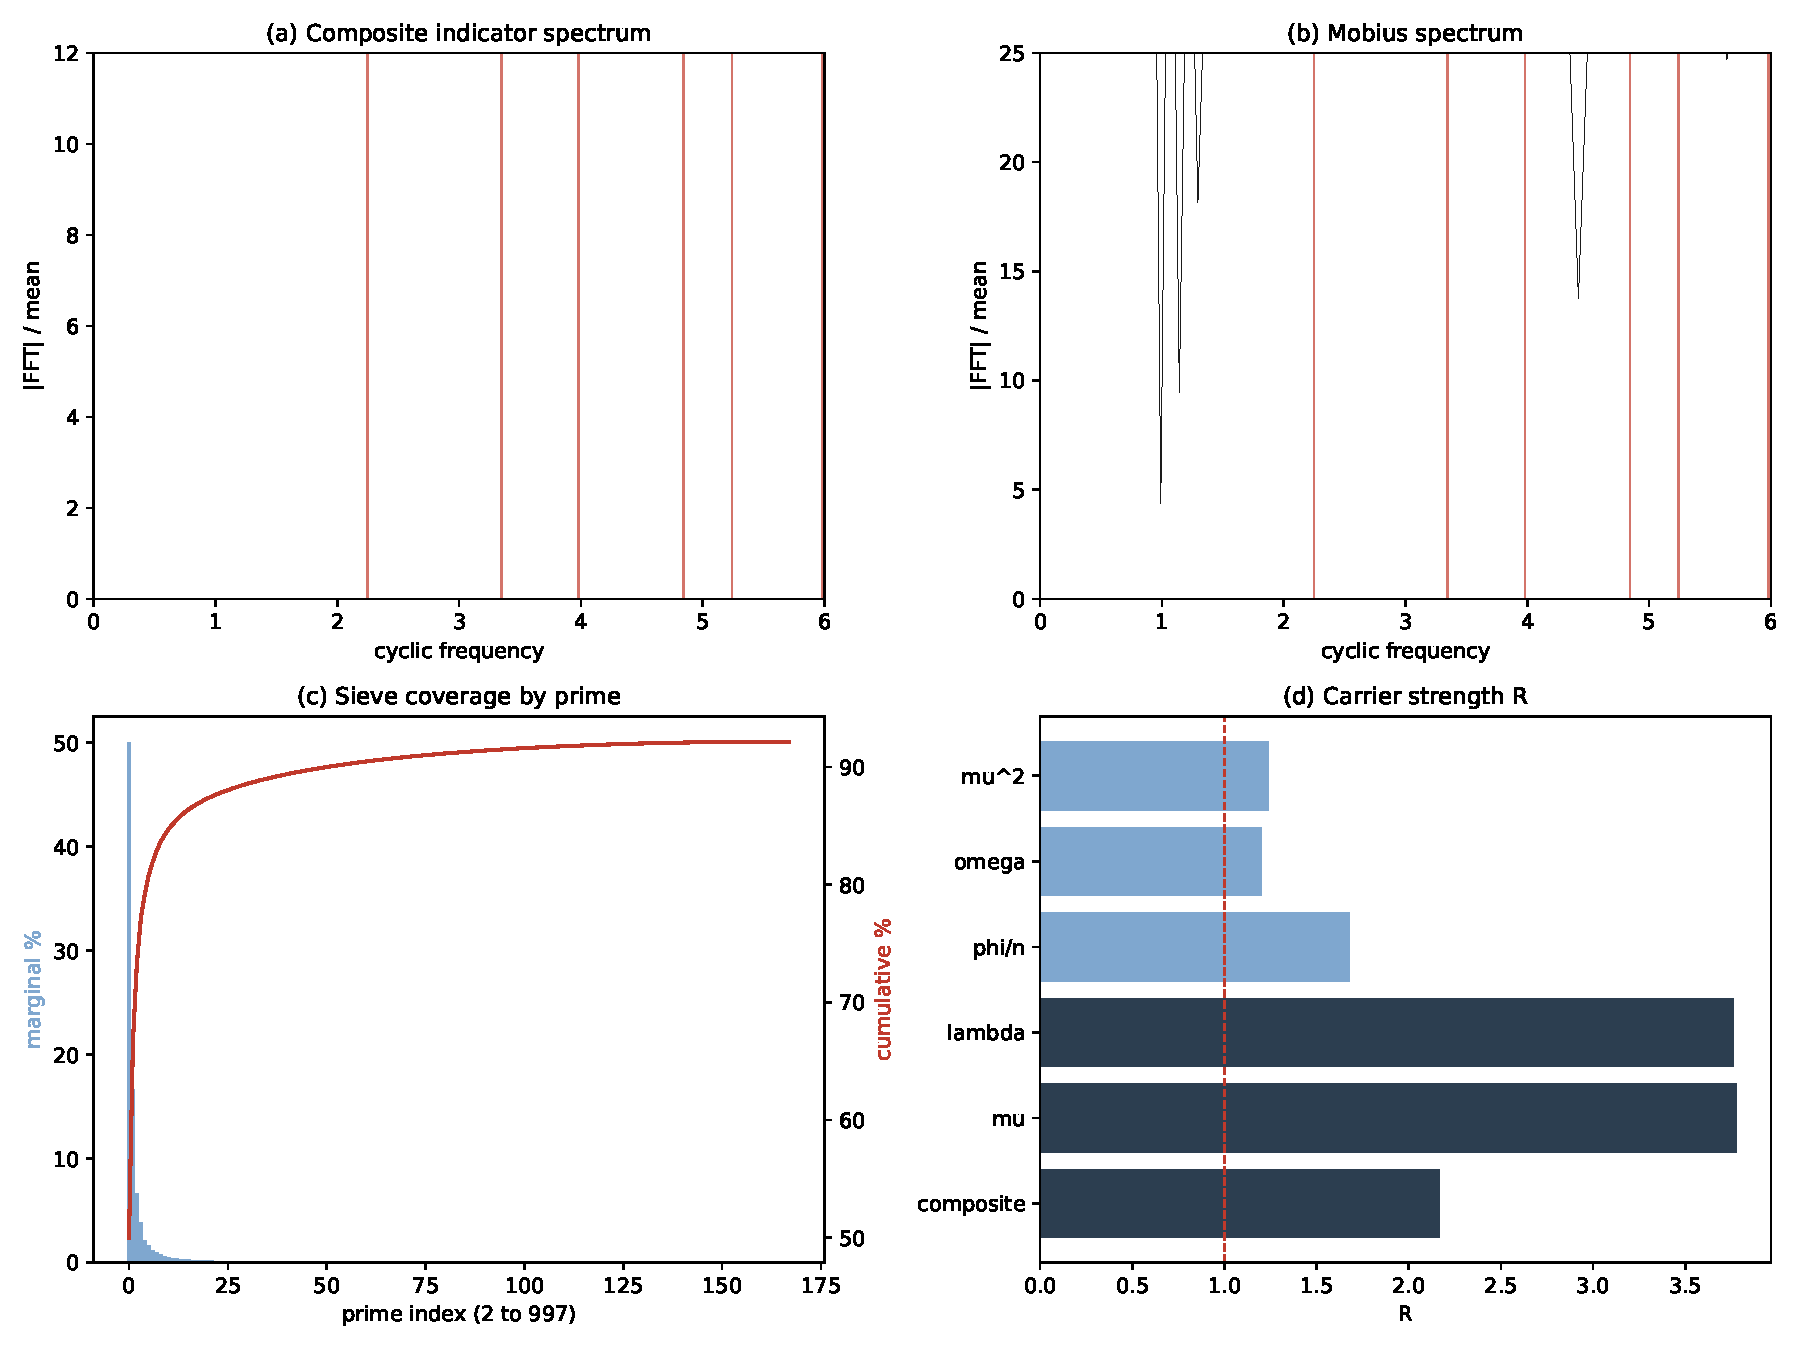
\includegraphics[width=\textwidth]{companion_sieve_flow_4panel.pdf}
\caption{The sieve-flow instrument. (a) Composite-indicator spectrum:
peaks at $\gamma_k/2\pi$ (red), $R=2.17$. (b) M\"obius spectrum:
same peaks, $R=3.78$. (c) Sieve coverage: marginal (blue bars) and
cumulative (red) fraction of $[2,10^6]$ first marked by each prime;
$2$ alone defines $50\%$. (d) Carrier strength $R$ across arithmetic
functions; dashed line is null.}
\label{fig:4panel}
\end{figure}

\section{The exact sieve backbone}

\begin{theorem}[Seed generation]\label{thm:seed}
The primes $\le\sqrt{N}$ generate the exact prime/composite bitmap
on $[2,N]$ by Eratosthenes.  The same seed computes $d(n)$,
$\mu(n)$, and $\lambda(n)$ for every $n\le N$.
\end{theorem}
\begin{proof}
Standard: $n\le N$ composite implies a prime factor $\le\sqrt{n}\le
\sqrt{N}$.  The divisor and M\"obius/Liouville values follow from
the prime factorization, which the sieve provides.
\end{proof}

At $N=10^6$, $168$ primes $\le 1000$ generate all $10^6$ bits;
$\pi(10^6)=78{,}498$ is recovered exactly, and the seed-generated
$D(10^6)=13{,}970{,}034$ matches the independent floor sum.

\section{The spectral pipeline}
Given an arithmetic pattern $b(n)$ on $[2,N]$:
\begin{enumerate}[label=(\arabic*)]
\item \emph{Log-resample:} $t=\log n$; interpolate $b$ onto a uniform
$t$-grid ($K=200{,}000$ points).  The explicit formula's
oscillations $x^{i\gamma}=e^{i\gamma t}$ are pure sinusoids in $t$.
\item \emph{Detrend:} subtract uniform-filter smoothing (window
$K/25$), then the mean.
\item \emph{FFT:} magnitude spectrum $\lvert\mathrm{FFT}\rvert$.
\item \emph{$R$ statistic:}
\[
R=\frac{\text{mean }\lvert\mathrm{FFT}\rvert\text{ in }\pm0.12
\text{ about }\gamma_k/2\pi,\ k=1..8}
{\text{mean }\lvert\mathrm{FFT}\rvert\text{ at gap midpoints}}.
\]
The target is $\gamma_k/2\pi$ (cyclic), not $\gamma_k$, since the
Fourier conjugate of $t=\log n$ is $1/\log$.
\end{enumerate}
$R\gg1$ means the zero spectrum is present; $R\approx1$ is null
(shuffled controls confirm).

A byte-verified reproducer is posted at
\texttt{research-notes/sieve\_flow\_R\_pipeline\_reproducer.py}.

\section{The carrier gradient}
\begin{center}
\begin{tabular}{lcl}
Pattern & $R$ & Dirichlet series \\ \hline
Composite indicator & $2.17$ & --- \\
$\mu(n)$ & $3.78$ & $1/\zeta(s)$ \\
$\lambda(n)$ & $3.76$ & $\zeta(2s)/\zeta(s)$ \\
$\phi(n)/n$ & $1.68$ & $\zeta(s-1)/\zeta(s)$ \\
$\omega(n),\Omega(n)$ & $\approx1.2$ & $\zeta(s)P(s)$ \\
$\mu^2(n)$ (squarefree) & $1.24$ at $\gamma/2$ & $\zeta(s)/\zeta(2s)$
\end{tabular}
\end{center}
The $R$-values rank by how cleanly the Dirichlet series isolates
$1/\zeta$-type poles.  Multiplicativity is a $\sim3\times$
amplifier, not a strict gate: additive seed-generated functions
($\omega,\Omega$) are weak but real carriers.

\section{The kills}
The instrument falsifies as readily as it confirms:
\begin{itemize}
\item \emph{$\chi_{12}$ twist:} $R_L=1.37$ at $10^6$ decays to
$1.08$ at $10^8$ (null).  Clean negative.
\item \emph{Twin primes:} $R\approx1.66$ at both $10^6$ and $10^7$;
seven times more data, no strengthening.
\item \emph{Small-prime weighting:} the binary prime indicator
carries $R=1.58$ (not the composite $2.17$); emphasizing small
primes weakens it ($1.58\to1.07$ for $1/\log p$, $1.58\to1.06$
for $1/\sqrt p$, both near null), while the von Mangoldt
($\log p$) weight strengthens it ($1.58\to2.55$).  Leverage is
in \emph{generation}, not weighting.
\end{itemize}

\section{Fold recursion and coverage}
$R$ is scale-free: $1.87\to2.01\to2.24\to2.17\to2.19$ for
$N=10^3,\dots,10^7$.  A single fold encloses all folds beneath it.

Coverage is front-loaded with no anomalous jumps (Figure~\ref{fig:4panel}(c)):
$2$ defines $50\%$, $+3$ reaches $66.7\%$, then smooth
$1/(p\log p)$ decay.  Since $2\cdot3=6$, every prime $>3$ is
$6\pm1$; mod $12$ refines this to the four classes
$\{1,5,7,11\}$, with $(\mathbb{Z}/12)^\times\cong V_4$ the
smallest modulus carrying Klein-four units.  The $V_4$ is forced
by the $\{2,3\}$-sieve dominance, not imposed.

\section{The distinguished hyperbola}
The $xy=n$ hyperbola is the \emph{unique} conic section carrying
the strong spectrum: it is the multiplication table itself, with
the fold at $\sqrt{n}$ as symmetry axis.  The encoding runs
through the \emph{binary fold decision} ($d(n)=2$ vs.\ $d(n)>2$,
$R=2.17$), not the raw lattice count ($R=1.16$).  The circle cut
$x^2+y^2=n$ gives $R=0.73$ (suppressed); only the unbounded
hyperbola, leaving the cone's boundary, encodes completely.

\bibliographystyle{plain}
\begin{thebibliography}{9}
\bibitem{ledger}
Cone Derivation Ledger, v13.942, v13.948, v13.952, v13.963, v13.983, v13.984,
\texttt{unified/discriminant-12-return/ledger/}.
\end{thebibliography}

\end{document}
